% ==============================================================================
% best_equipo_01.tex
% Presentación "Best Model Deep Dive": la historia del mejor modelo, desde los
% datos hasta la decisión de compra. Las diapositivas c01 a c13 de comunes/
% también están en compare_equipo_01.tex.
% Compilar desde esta carpeta: pdflatex best_equipo_01.tex (dos veces).
% ==============================================================================
\documentclass[aspectratio=169, 11pt]{beamer}
% ==============================================================================
% preambulo.tex
% Preámbulo común de las dos presentaciones (best_equipo_01 y compare_equipo_01).
% Las figuras y tablas se toman de 03_Output, donde las generan los scripts del
% repositorio, y las cifras citadas vienen de 03_Output/Tables/pres_cifras.tex
% (01_Scripts/04_Results/03_figuras_presentaciones.R).
% ==============================================================================
\usepackage[T1]{fontenc}
\usepackage[utf8]{inputenc}
\usepackage{lmodern}
\usepackage{graphicx}
\usepackage{booktabs}
\usepackage{tikz}
\usetikzlibrary{positioning, arrows.meta}

\graphicspath{{../03_Output/Figures/}}
\newcommand{\maeprivado}{151,5}
\newcommand{\preciotipico}{806}
\newcommand{\maepctprecio}{19\%}
\newcommand{\ntrain}{36.407}
\newcommand{\nrawtrain}{38.644}
\newcommand{\ncopias}{2.237}
\newcommand{\ntest}{10.286}
\newcommand{\nchaptrain}{305}
\newcommand{\pcttestchap}{94\%}
\newcommand{\preciomdchap}{750}
\newcommand{\preciomdresto}{550}
\newcommand{\aptotest}{97\%}
\newcommand{\aptotrain}{75\%}
\newcommand{\sinareatest}{44\%}
\newcommand{\sinareachap}{6\%}
\newcommand{\coordredondeada}{52\%}
\newcommand{\coordredtrain}{40\%}
\newcommand{\nvarexternas}{61}
\newcommand{\nvartexto}{44}
\newcommand{\ntopicos}{15}
\newcommand{\nenvios}{25}
\newcommand{\margenchap}{19\%}
\newcommand{\sobreestimachap}{46\%}
\newcommand{\sobrediezchap}{25\%}
\newcommand{\pctverde}{11\%}
\newcommand{\pctamarillo}{61\%}
\newcommand{\pctrojo}{27\%}
\newcommand{\mejormargen}{17\%}
\newcommand{\gananciacien}{1.153}
\newcommand{\negociosmargen}{42\%}
\newcommand{\descuentomax}{15\%}
\newcommand{\pasoentorno}{96}
\newcommand{\pasoxgb}{37}
\newcommand{\pasotexto}{13}
\newcommand{\ventajaxgb}{39}
\newcommand{\ventajaensamble}{3}
\newcommand{\mismabasedif}{58}
\newcommand{\cartdistintos}{59}
\newcommand{\sesgobarato}{17\%}
\newcommand{\sesgocaro}{19\%}


% Colores
\definecolor{azul}{HTML}{2166AC}
\definecolor{rojo}{HTML}{B2182B}
\definecolor{verde}{HTML}{1A9850}
\definecolor{gris}{HTML}{595959}
\definecolor{grisclaro}{HTML}{F2F2F2}

% Tema sobrio: títulos en azul, sin íconos de navegación, número de página
\usetheme{default}
\setbeamertemplate{navigation symbols}{}
\setbeamercolor{frametitle}{fg=azul}
\setbeamerfont{frametitle}{series=\bfseries, size=\large}
\setbeamercolor{title}{fg=azul}
\setbeamerfont{title}{series=\bfseries}
\setbeamercolor{structure}{fg=azul}
\setbeamertemplate{itemize items}[circle]
\setbeamertemplate{footline}{%
  \hfill\textcolor{gris}{\scriptsize Equipo 1 \quad \insertframenumber/\inserttotalframenumber}\hspace{1em}\vspace{0.6em}}

% Cifra grande con su descripción. El argumento opcional es el ancho (por
% defecto, un tercio del ancho de la diapositiva).
\newcommand{\cifra}[3][0.3\textwidth]{%
  \begin{minipage}[t]{#1}\centering
    {\Huge\bfseries\color{azul}#2}\\[0.3em]
    {\small\color{gris}#3}
  \end{minipage}}

% Cifra mediana, para acompañar un mapa sin quitarle espacio
\newcommand{\cifrachica}[2]{%
  {\LARGE\bfseries\color{azul}#1}\\[0.1em]
  {\footnotesize\color{gris}#2}}

% Mensaje corto debajo de una figura
\newcommand{\lectura}[1]{\par\vspace{0.2em}{\scriptsize\color{gris}#1}}

% Diapositivas de mapa vertical: el mapa ocupa toda la altura a la izquierda y
% el título va arriba de la columna derecha, con el mismo estilo de los demás
% títulos. \altomapa es la altura del mapa.
\newcommand{\altomapa}{1.02\textheight}
\newcommand{\titulolateral}[1]{%
  {\usebeamerfont{frametitle}\usebeamercolor[fg]{frametitle}#1\par}\vspace{0.9em}}
\newcommand{\mapavertical}[1]{\vspace*{-0.4em}\includegraphics[height=\altomapa]{#1}}

% Figura ancha que usa casi todo el ancho de la diapositiva
\newcommand{\figuraancha}[2][0.97]{\makebox[\textwidth]{\includegraphics[width=#1\paperwidth]{#2}}}


\title{¿Le confiaríamos la plata a este modelo?}
\subtitle{Precios de vivienda en Chapinero: del mejor modelo a la decisión de compra}
\author{Equipo 1: Mauricio Aragón, Jonathan Cadena y Esteban Flórez}
\date{Big Data y Machine Learning para Economía Aplicada (MECA 4107)\\Universidad de los Andes, 2026-20}

\begin{document}

\begin{frame}[plain]
  \titlepage
\end{frame}

% --- El mejor modelo y el problema --------------------------------------------
% C1. Resultado del mejor modelo (inicio obligatorio de las dos presentaciones)
\begin{frame}{El mejor modelo se equivoca en \maeprivado{} millones por vivienda}
  \centering
  \cifra{\maeprivado{} M}{MAE privado en Kaggle\\(envío 29, ensamble de XGBoost)}\hfill
  \cifra{\maepctprecio}{del precio típico predicho\\en Chapinero (\preciotipico{} M)}\hfill
  \cifra{\nenvios}{envíos a Kaggle con\\seis familias de algoritmos}

  \vspace{1.6em}
  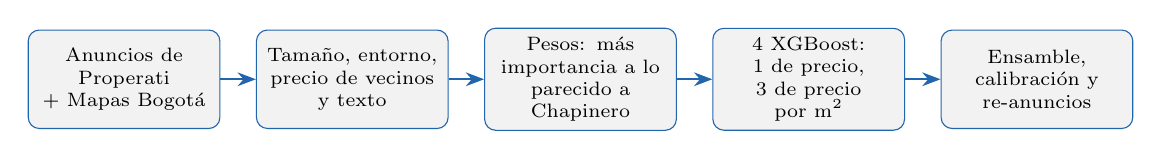
\begin{tikzpicture}[node distance=0.45cm,
      caja/.style={draw=azul, fill=grisclaro, rounded corners, align=center,
                   font=\scriptsize, minimum height=1.25cm, text width=2.2cm},
      flecha/.style={-{Stealth}, thick, azul}]
    \node[caja] (datos) {Anuncios de\\Properati\\+ Mapas Bogotá};
    \node[caja, right=of datos] (vars) {Tamaño, entorno,\\precio de vecinos\\y texto};
    \node[caja, right=of vars] (pesos) {Pesos: más\\importancia a lo\\parecido a Chapinero};
    \node[caja, right=of pesos] (xgb) {4 XGBoost:\\1 de precio,\\3 de precio\\por m$^2$};
    \node[caja, right=of xgb] (ens) {Ensamble,\\calibración y\\re-anuncios};
    \draw[flecha] (datos) -- (vars);
    \draw[flecha] (vars) -- (pesos);
    \draw[flecha] (pesos) -- (xgb);
    \draw[flecha] (xgb) -- (ens);
  \end{tikzpicture}
  \note{El MAE es el error absoluto medio: en promedio el precio predicho se aleja \maeprivado{} millones del precio de venta, cerca de \maepctprecio{} del precio típico. El modelo combina cuatro XGBoost: uno predice el precio y tres el precio por metro cuadrado. El envío también probó agregar modelos con embeddings del texto, pero el ensamble les dio un peso de casi cero, así que en la práctica es un ensamble de XGBoost. Los pesos hacen que el modelo aprenda más de los anuncios parecidos a los de Chapinero. Los re-anuncios son viviendas de test que ya aparecían en train con otra publicación.}
\end{frame}

% C2. El reto: train en toda Bogotá, test en Chapinero
\begin{frame}{El reto: predecir donde casi no hay datos}
  \begin{columns}[c]
    \begin{column}{0.5\textwidth}\centering
      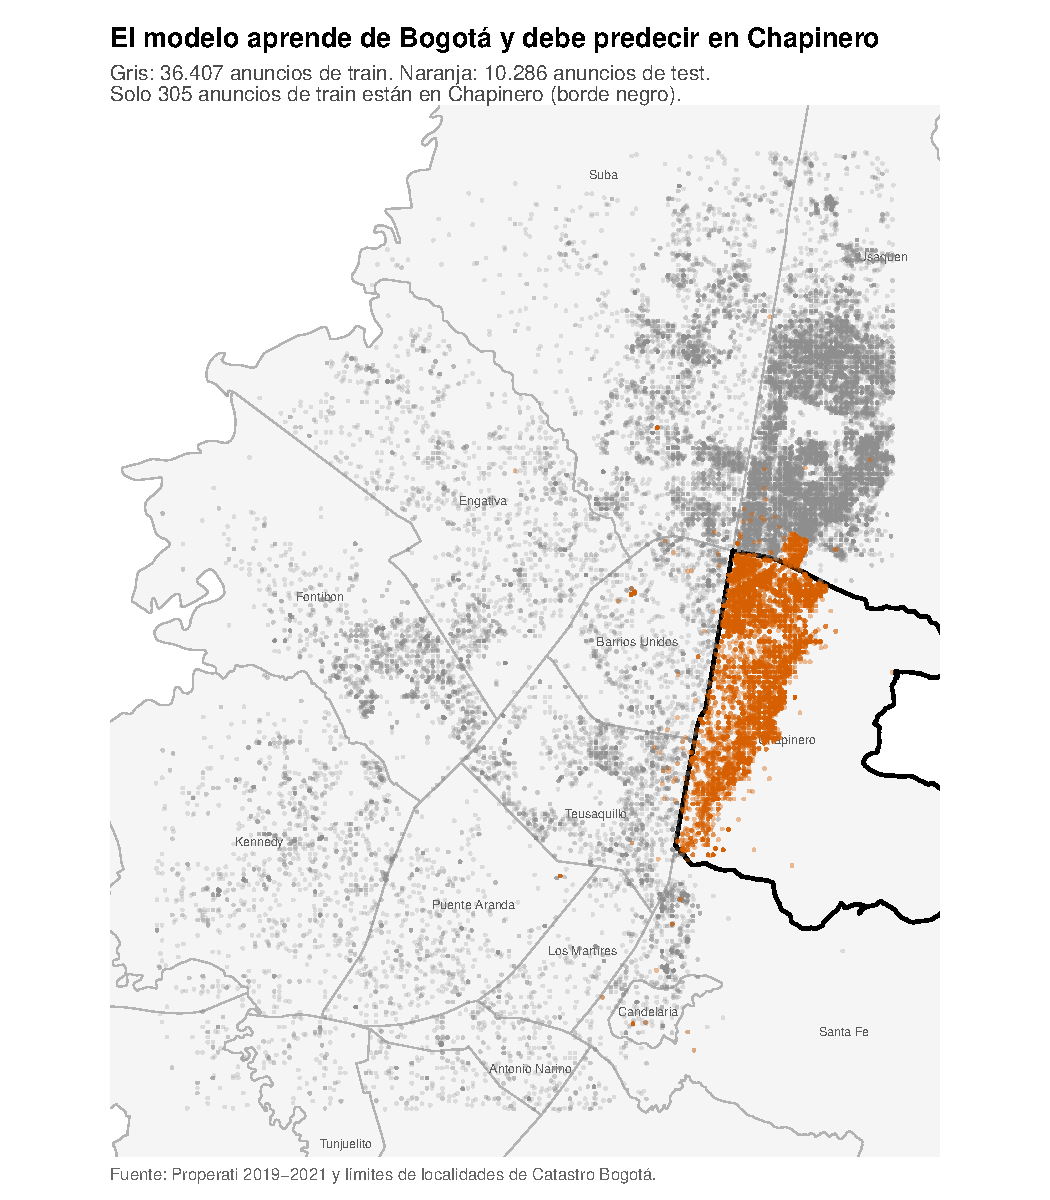
\includegraphics[height=0.82\textheight]{mapa_01_train_test.pdf}
    \end{column}
    \begin{column}{0.45\textwidth}
      \cifra[\linewidth]{\ntrain}{anuncios de train en toda Bogotá}\\[1.2em]
      \cifra[\linewidth]{\nchaptrain}{de ellos en Chapinero}\\[1.2em]
      \cifra[\linewidth]{\pcttestchap}{de los \ntest{} anuncios de test están en Chapinero}
    \end{column}
  \end{columns}
  \note{La empresa quiere comprar en Chapinero, pero los datos para aprender son de toda la ciudad. El modelo tiene que extrapolar: aprender en Suba, Kennedy o Usaquén y predecir en Chapinero. Por eso la validación cruzada aleatoria no basta, y por eso usamos validación espacial.}
\end{frame}

% C3. Chapinero es más caro y tiene peor información
\begin{frame}
  \begin{columns}[c]
    \begin{column}{0.6\textwidth}\centering
      \mapavertical{mapa_02_precio_m2_upz.pdf}
    \end{column}
    \begin{column}{0.38\textwidth}
      \titulolateral{Chapinero es más caro, casi todo apartamentos y con ubicación más imprecisa}
      \resizebox{\linewidth}{!}{%
      \begin{tabular}{@{}lrr@{}}
        \toprule
        & Chapinero & Bogotá \\
        \midrule
        Precio mediano (M)$^{*}$ & \preciomdchap & \preciomdresto \\
        Apartamentos & \aptotest & \aptotrain \\
        Coordenadas redondeadas & \coordredondeada & \coordredtrain \\
        \bottomrule
      \end{tabular}}

      \vspace{0.6em}
      {\scriptsize\color{gris}Apartamentos y coordenadas: test (Chapinero) frente a train (Bogotá). $^{*}$ Test no tiene precio: se compara Chapinero con el resto de Bogotá, ambos en train.\par}

      \vspace{0.6em}
      {\scriptsize\color{gris}Coordenadas redondeadas: con 3 decimales o menos, un error de ubicación de unos 110 m.\par}
    \end{column}
  \end{columns}
  \note{Chapinero está entre las zonas más caras de la ciudad. En test casi todo son apartamentos, y la ubicación es menos precisa: más de la mitad de las coordenadas viene redondeada. Además, al \sinareatest{} de test le falta el área, frente a solo el \sinareachap{} de los anuncios de Chapinero que sí están en train.}
\end{frame}

% C4. Qué le agregamos a los datos
\begin{frame}
  \begin{columns}[c]
    \begin{column}{0.6\textwidth}\centering
      \mapavertical{mapa_09_contexto_urbano.pdf}
    \end{column}
    \begin{column}{0.38\textwidth}
      \titulolateral{Qué le agregamos a los datos: el entorno y lo que dice el anuncio}
      {\footnotesize\textbf{\color{azul}\nvarexternas{} variables externas} (Mapas Bogotá, Catastro)}
      \begin{itemize}\scriptsize
        \item Valor de referencia del suelo, avalúos y estrato por manzana
        \item TransMilenio, metro, SITP y ciclorrutas
        \item Parques, árboles, colegios, IPS, comercio y restaurantes
        \item Riesgo y elevación
      \end{itemize}
      {\footnotesize\textbf{\color{azul}\nvartexto{} variables del texto}}
      \begin{itemize}\scriptsize
        \item Área, baños, parqueaderos y piso escritos en el anuncio
        \item Palabras clave (terraza, gimnasio, lujo) y barrios
        \item Lasso sobre las palabras y \ntopicos{} tópicos (LDA)
      \end{itemize}
    \end{column}
  \end{columns}
  \note{El enunciado pide al menos cuatro variables externas y cuatro de texto; tenemos muchas más. Las externas vienen de las capas de Mapas Bogotá y de Catastro. Del texto sacamos números que no estaban en las columnas (área, baños) y también usamos el texto como datos: un Lasso que predice el precio con las palabras y tópicos que resumen de qué habla cada anuncio. Aparte de estos dos grupos, el modelo usa el precio por metro cuadrado de los anuncios vecinos en train (rezago espacial), que no viene de una fuente externa.}
\end{frame}

% C5. Qué revela el modelo sobre los precios (interpretación hedónica)
\begin{frame}{Qué revela el modelo: el precio es tamaño, ubicación y lo que dice el anuncio}
  \centering
  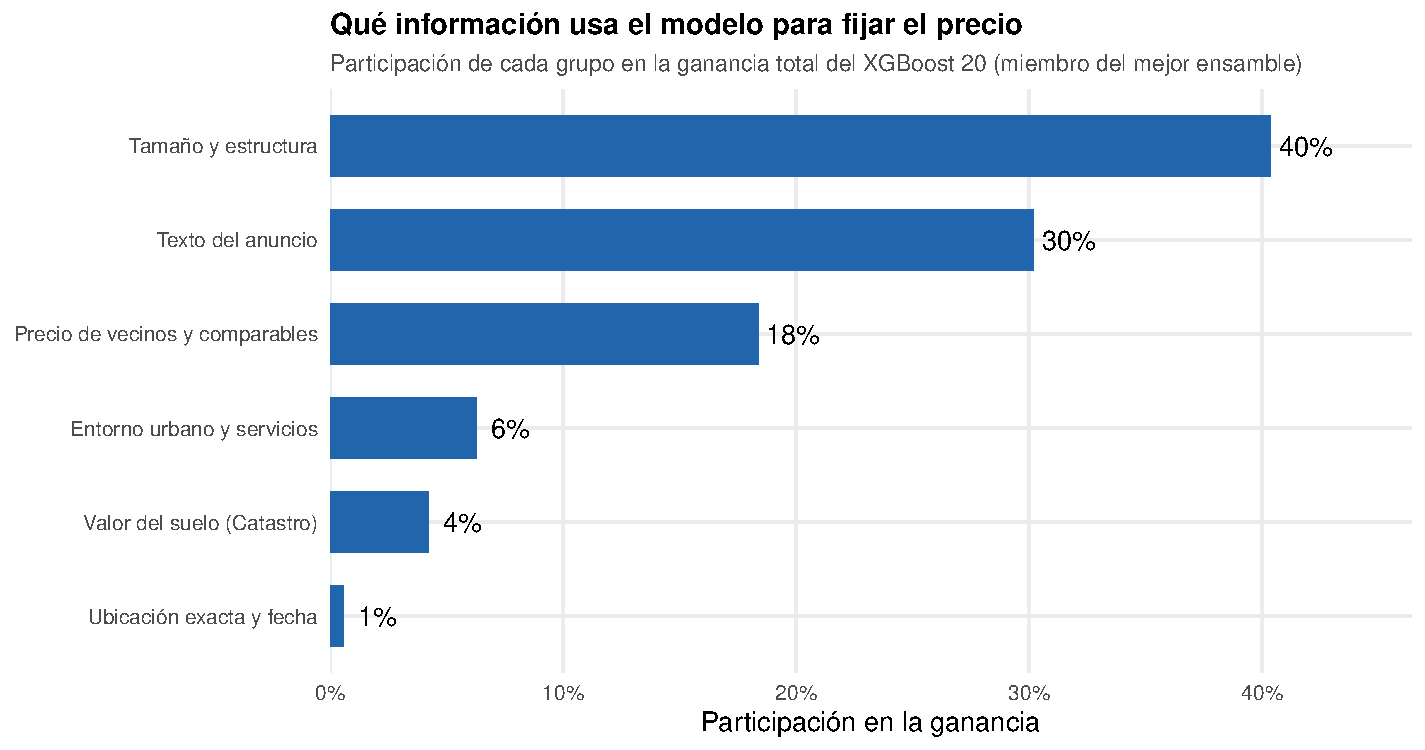
\includegraphics[height=0.8\textheight]{pres_importancia_grupos.pdf}
  \lectura{Como en Rosen (1974), el precio depende de las características de la vivienda y de su entorno. El texto recoge calidad y acabados que ninguna otra variable mide.}
  \note{La ganancia mide cuánto mejora el ajuste cada vez que el modelo usa una variable. El tamaño (área, baños, habitaciones) explica el nivel del precio. El texto es el segundo grupo: dice si el inmueble es de lujo, está remodelado o tiene club house. El precio de los vecinos y el valor del suelo de Catastro resumen la ubicación. Las amenidades sueltas (parques, transporte) pesan poco por separado, porque su efecto ya está en el precio de la zona.}
\end{frame}

% C6. Escalera del error
\begin{frame}{Cada idea, cuánto bajó el error: los datos importaron más que el algoritmo}
  \centering
  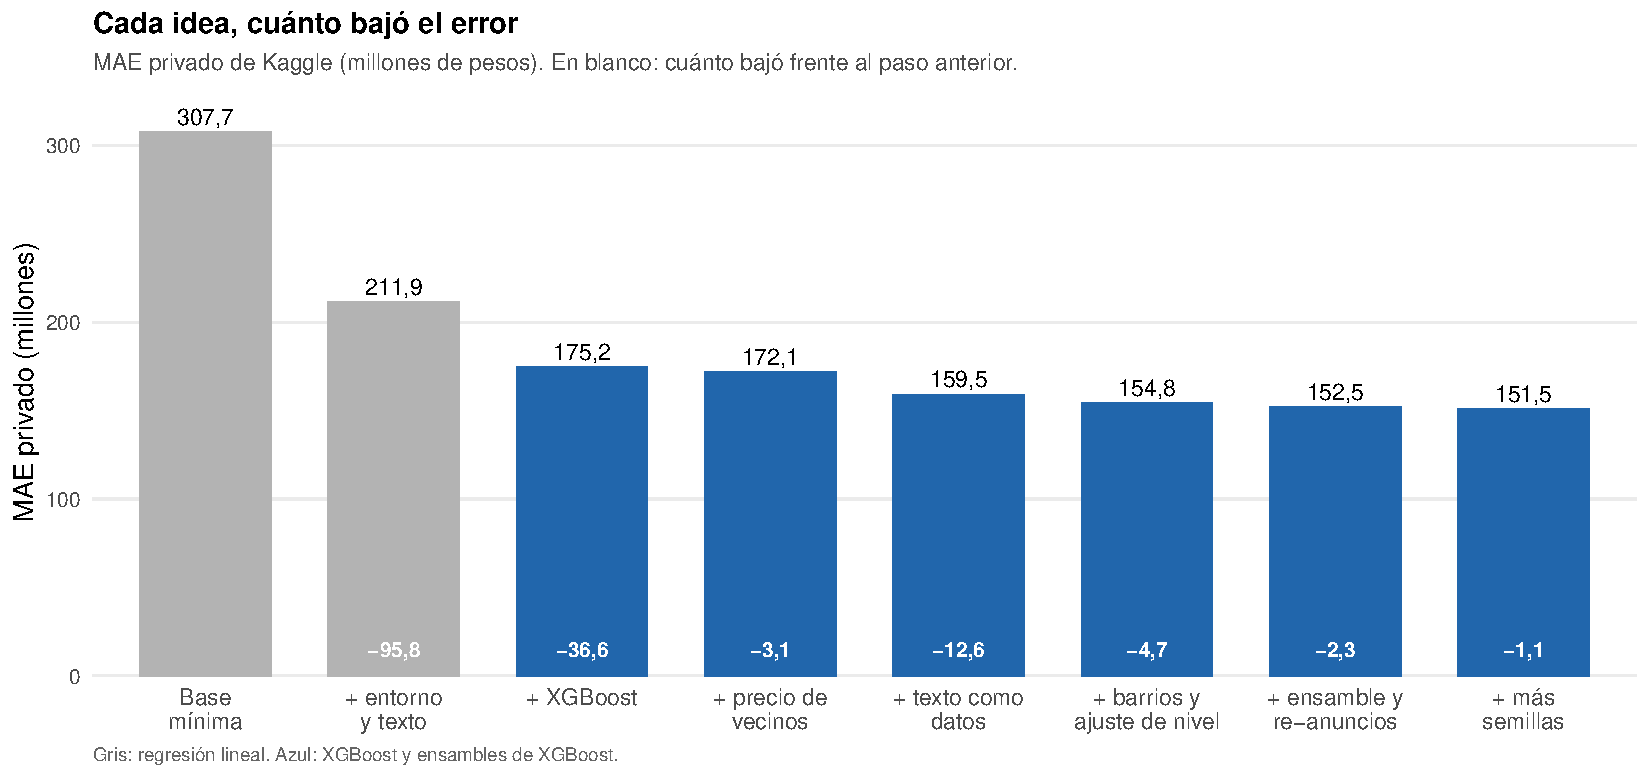
\includegraphics[width=\textwidth]{pres_escalera.pdf}
  \note{Pasar de una base mínima a la base con entorno y texto bajó el error \pasoentorno{} millones. Cambiar la regresión lineal por XGBoost, \pasoxgb{} millones. Después, el texto como datos fue el salto más grande (\pasotexto{} millones). El ensamble, los modelos del precio por m$^2$, las semillas y el ajuste de nivel aportan menos, pero suman. Los embeddings del último paso casi no recibieron peso en el ensamble.}
\end{frame}

% C7. Validación espacial
\begin{frame}{Cómo validamos: el modelo se evalúa en zonas de Bogotá que no vio}
  \centering
  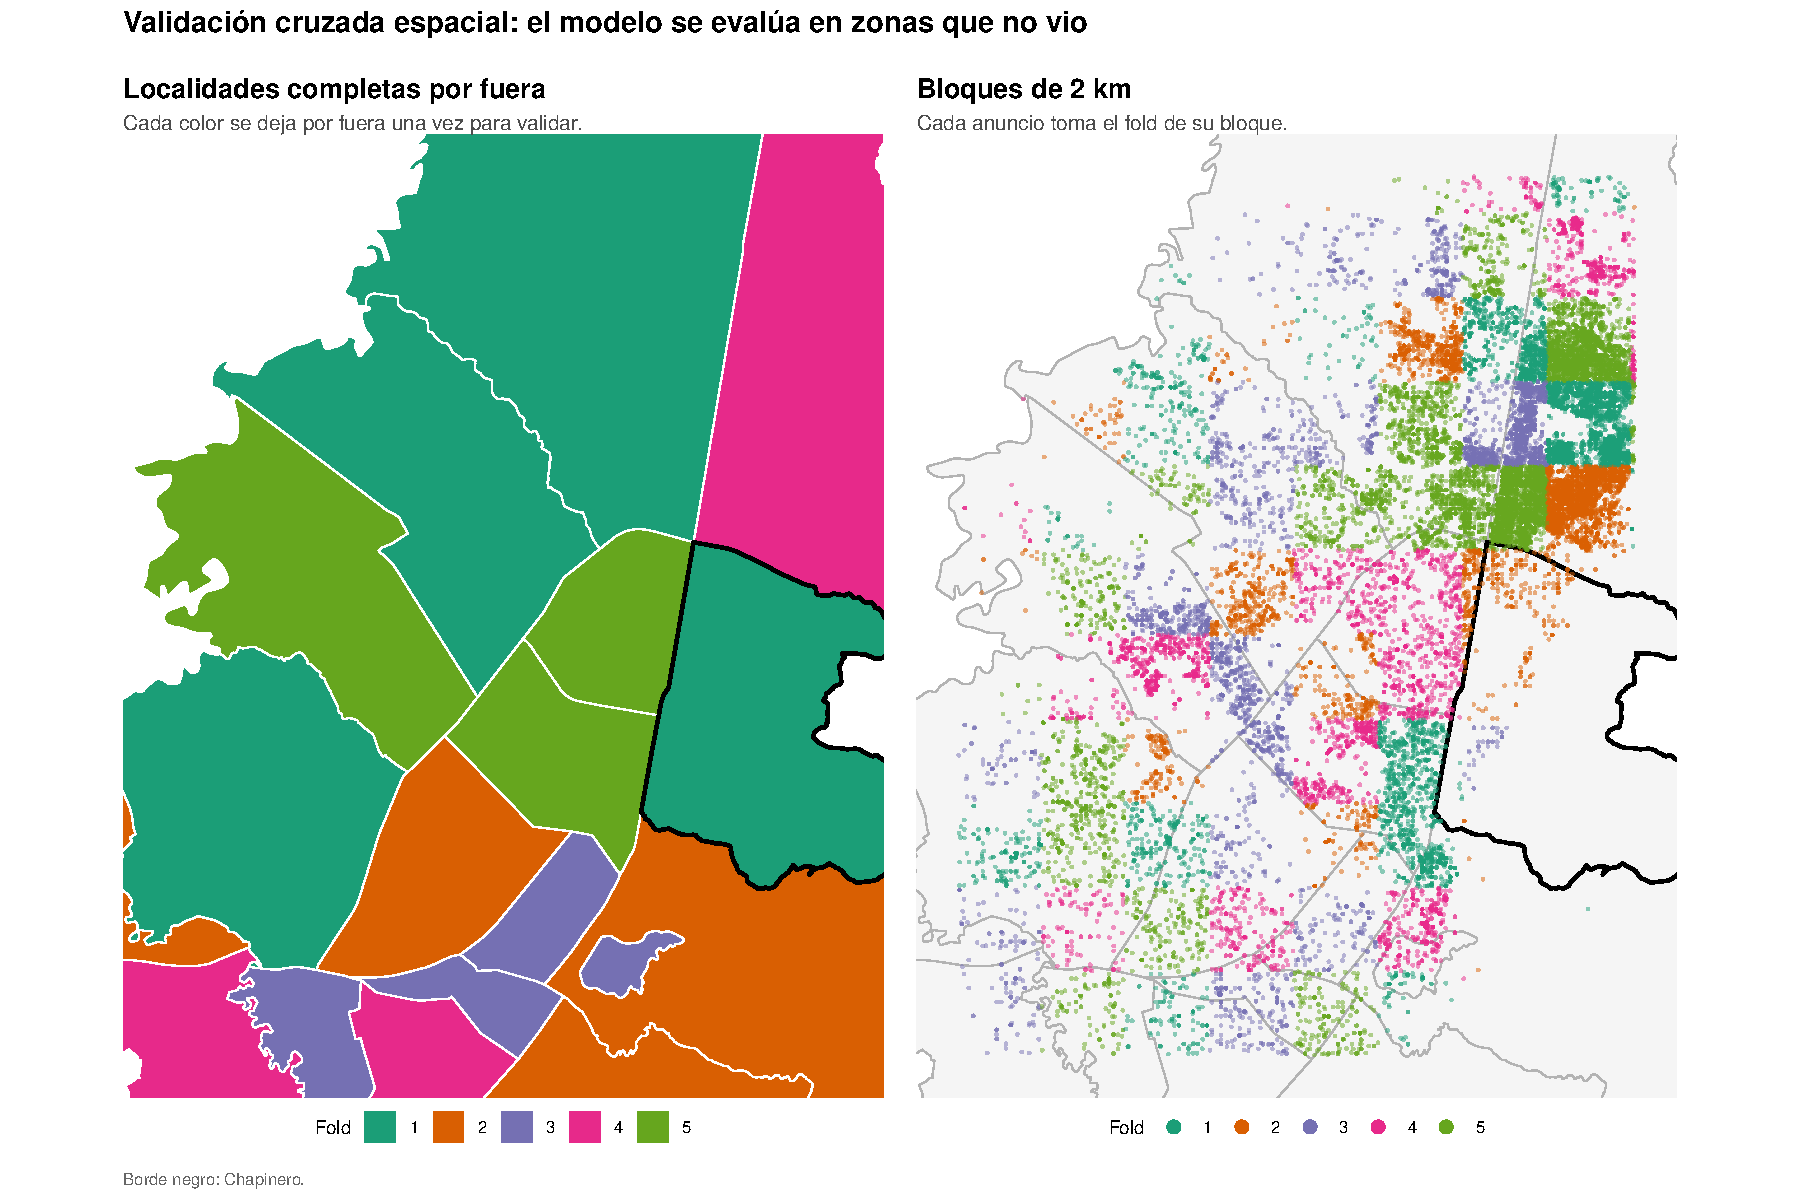
\includegraphics[height=0.86\textheight]{mapa_06_folds_espaciales.pdf}
  \note{En la validación aleatoria, un anuncio de validación casi siempre tiene vecinos en entrenamiento que comparten su precio, y el error se ve más bajo de lo que es. Con localidades completas por fuera, el modelo tiene que predecir una zona que no vio, como pasa con Chapinero. También probamos bloques de 2 km y bloques con un buffer de 300 metros.}
\end{frame}

% C8. Pesos por parecido con test
\begin{frame}{Le enseñamos al modelo a mirar lo que se parece a Chapinero}
  \begin{columns}[c]
    \begin{column}{0.5\textwidth}\centering
      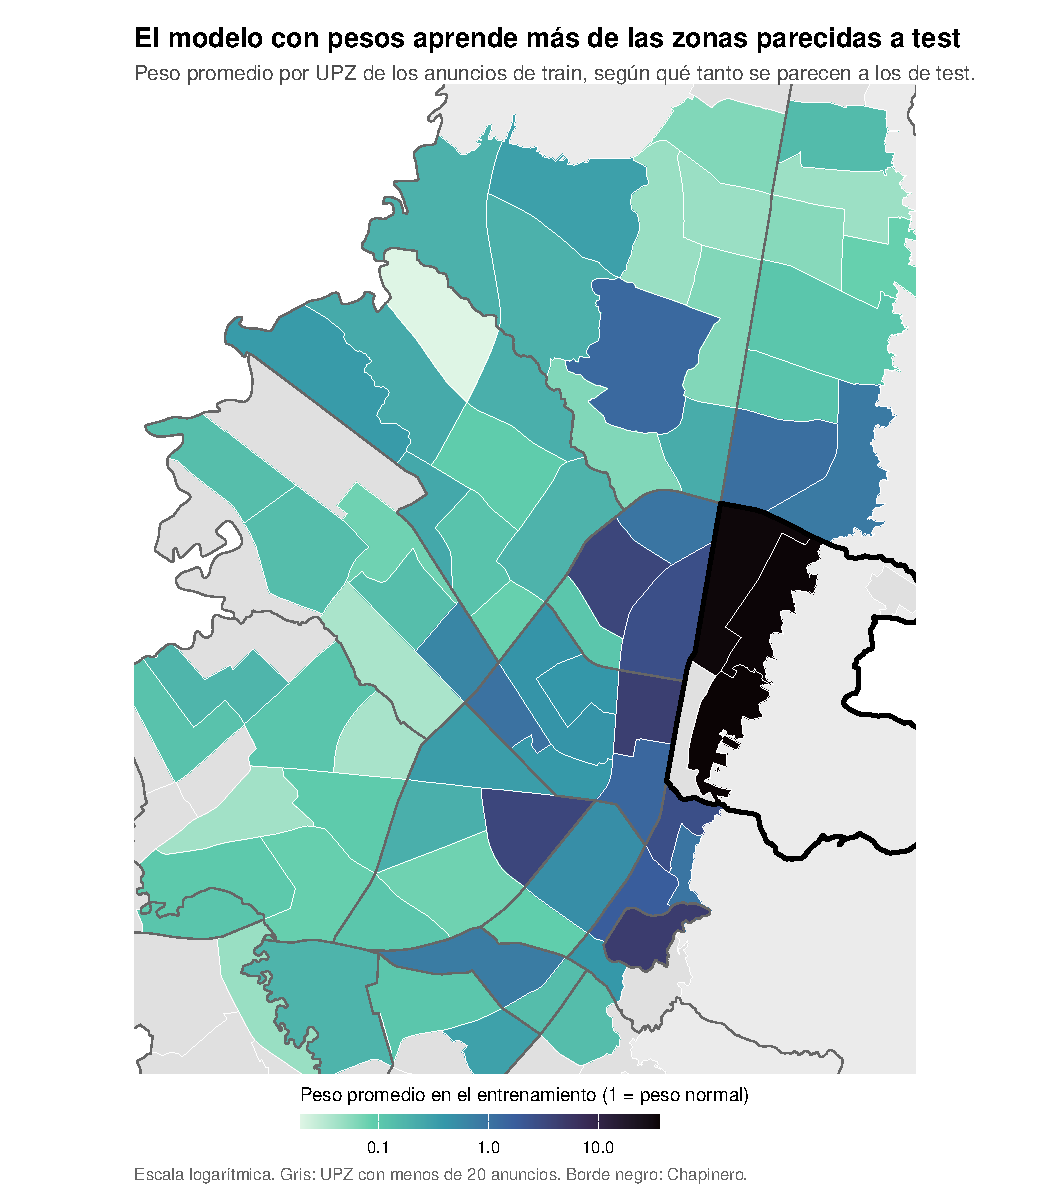
\includegraphics[height=0.82\textheight]{mapa_08_pesos_upz.pdf}
    \end{column}
    \begin{column}{0.45\textwidth}
      \begin{itemize}
        \item Un modelo aprende a distinguir los anuncios de train de los de test.
        \item Los anuncios de train que ``parecen de test'' reciben más peso al entrenar.
        \item Así el modelo dedica más esfuerzo a acertar en viviendas como las de Chapinero.
      \end{itemize}
    \end{column}
  \end{columns}
  \note{Es una forma de corregir el cambio de distribución entre train y test. El peso es la probabilidad de parecerse a test sobre la probabilidad de parecerse a train. En Kaggle los pesos ayudaron unos 3 millones en algunos pares de modelos, pero en el puntaje privado la ganancia no siempre se mantuvo: son diferencias pequeñas.}
\end{frame}


% --- Qué tan bien predice en Chapinero ----------------------------------------
\begin{frame}
  \begin{columns}[c]
    \begin{column}{0.6\textwidth}\centering
      \mapavertical{mapa_03_chapinero_prediccion_test.pdf}
    \end{column}
    \begin{column}{0.38\textwidth}
      \titulolateral{El modelo distingue zonas dentro de Chapinero}
      \begin{itemize}\footnotesize
        \item Precios por m$^2$ más altos en el norte (Chicó Lago) y en El Refugio.
        \item Más bajos en Chapinero central y hacia el sur.
        \item El modelo no le pone a toda la localidad el mismo precio: usa la cuadra, los vecinos y el anuncio.
      \end{itemize}
    \end{column}
  \end{columns}
  \note{Cada punto es un anuncio de test, con el precio por metro cuadrado que predice el envío 29. No es el precio observado, porque test no tiene precio. Se muestran solo los anuncios con área observada.}
\end{frame}

\begin{frame}
  \begin{columns}[c]
    \begin{column}{0.6\textwidth}\centering
      \mapavertical{mapa_04_chapinero_error_oof.pdf}
    \end{column}
    \begin{column}{0.38\textwidth}
      \titulolateral{Dónde se equivoca el modelo en Chapinero}
      \begin{itemize}\footnotesize
        \item Rojo: el modelo sobreestima el precio; azul: lo subestima.
        \item En Chapinero sobreestima el \sobreestimachap{} de las viviendas, y en más de 10\% el \sobrediezchap.
      \end{itemize}
    \end{column}
  \end{columns}
  \note{Estos errores son de anuncios de train predichos sin ver su localidad: es la mejor aproximación al error en test, porque en test no conocemos el precio. El error no se concentra en una sola zona: hay rojos y azules mezclados en toda la localidad.}
\end{frame}

\begin{frame}{Para ofertar importa el error según la predicción, y ahí casi no hay sesgo}
  \centering
  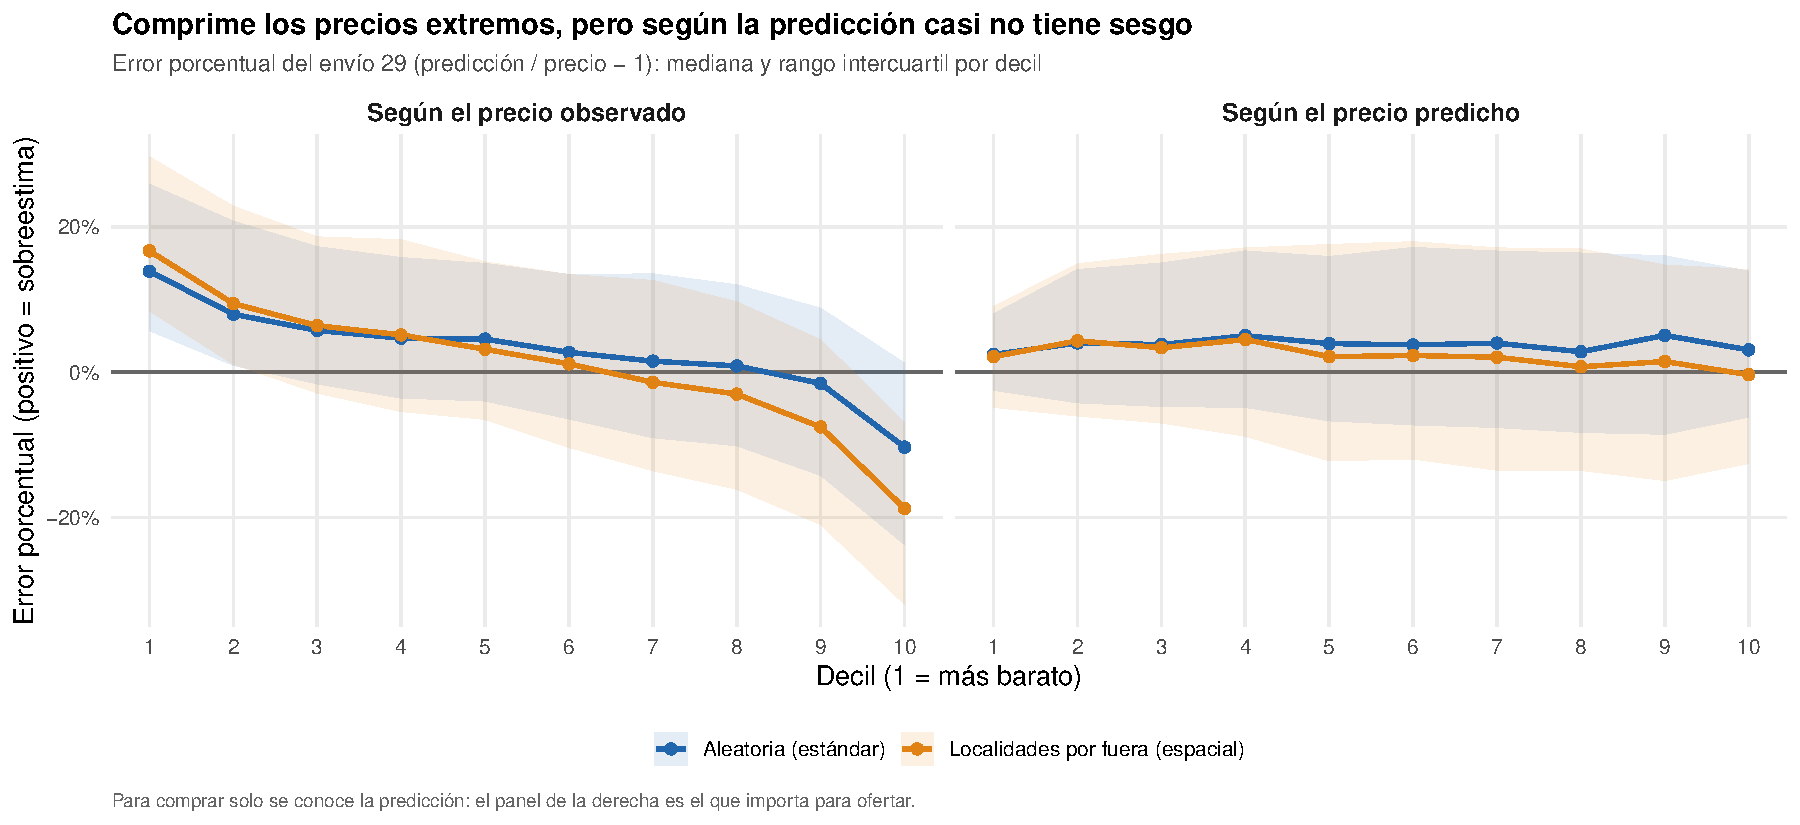
\includegraphics[height=0.74\textheight]{pres_sesgo_deciles.pdf}
  \lectura{Según el precio real, sobreestima lo más barato (\sesgobarato) y subestima lo más caro (\sesgocaro). Según la predicción, lo único que se conoce al ofertar, el error mediano es casi cero: el riesgo es la dispersión, no un sesgo.}
  \note{Aleatoria es la validación cruzada estándar, con los anuncios repartidos al azar; localidades es la validación cruzada espacial, con una localidad completa por fuera. Condicionar en el precio real siempre muestra regresión a la media: los modelos que predicen la media comprimen los extremos. Pero la empresa no conoce el precio real cuando oferta, solo la predicción. Dada la predicción, el modelo no está sesgado; lo que hay que cubrir es la dispersión (las bandas), y eso es lo que hace el margen de seguridad.}
\end{frame}

\begin{frame}
  \begin{columns}[c]
    \begin{column}{0.6\textwidth}\centering
      \mapavertical{mapa_05_chapinero_cobertura.pdf}
    \end{column}
    \begin{column}{0.38\textwidth}
      \titulolateral{Dónde el modelo tiene poca información para predecir}
      \begin{itemize}\scriptsize
        \item Azul: muchos anuncios de train cerca; el modelo tiene con qué comparar.
        \item Rojo: casi ninguno; el modelo extrapola desde otras zonas.
        \item La incertidumbre no es igual en toda la localidad: hay que tenerla en cuenta al ofertar.
      \end{itemize}
    \end{column}
  \end{columns}
  \note{Contamos cuántos anuncios de train hay a menos de 500 metros de cada anuncio de test. Las zonas con pocos vecinos son donde el error puede ser mayor, aunque el MAE promedio no lo muestre.}
\end{frame}

% --- Del modelo al negocio ----------------------------------------------------
% C9. Kaggle frente a negocio
\begin{frame}{Lo que gana en Kaggle no es lo que gana la empresa}
  \centering
  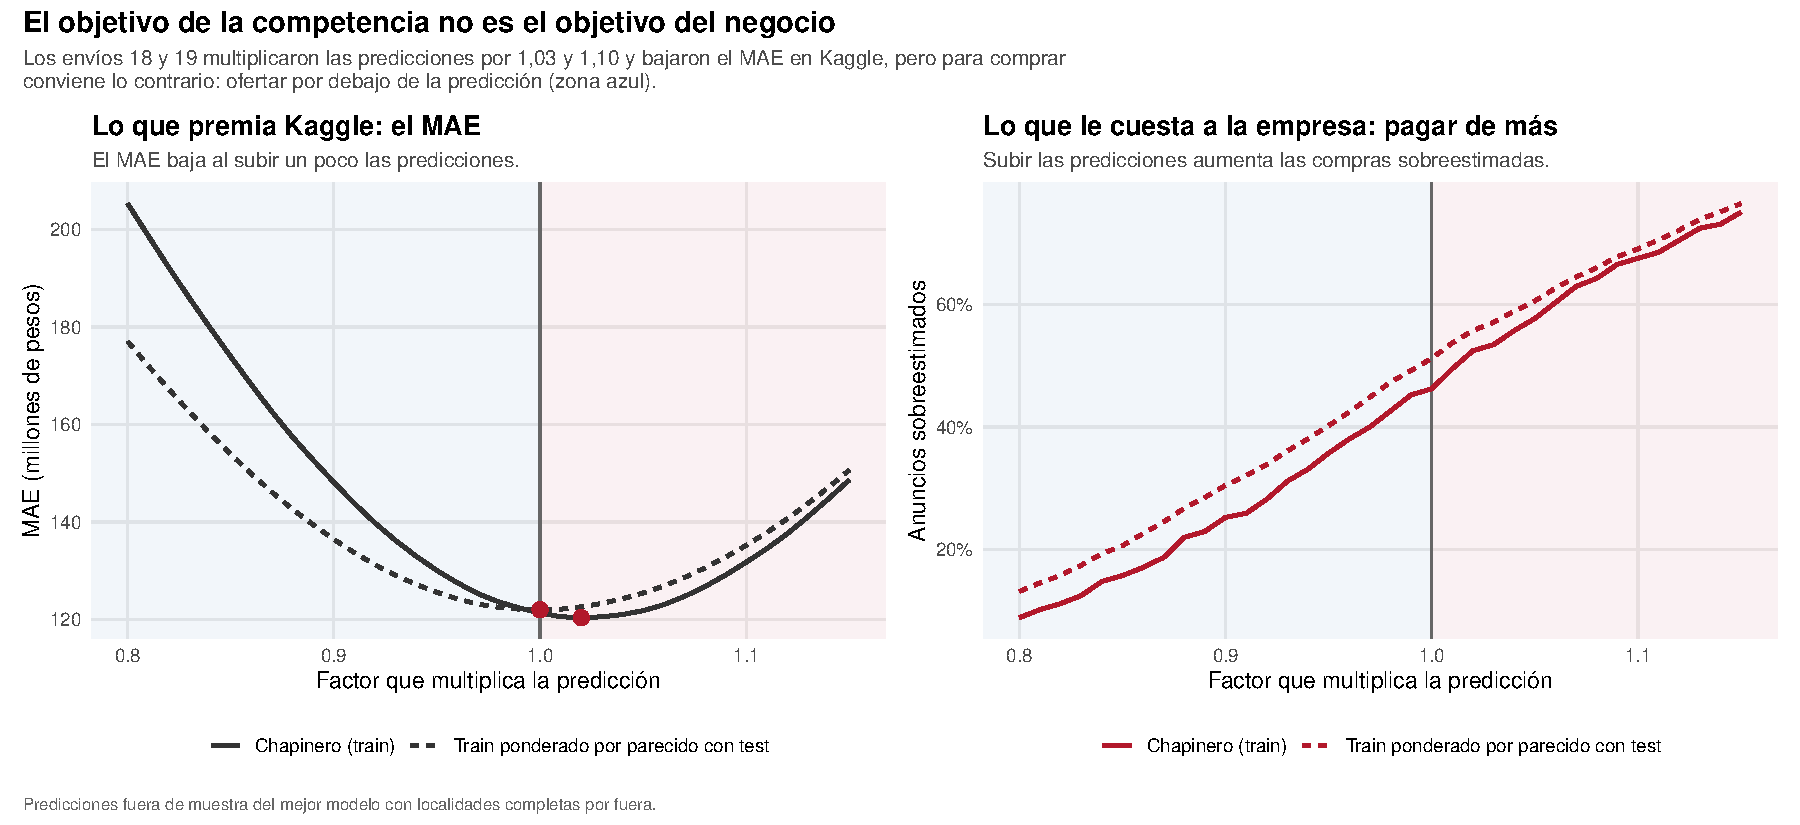
\includegraphics[width=\textwidth]{negocio_05_kaggle_vs_negocio.pdf}
  \note{El modelo subestima Chapinero, así que subir un poco las predicciones bajó el MAE en Kaggle. Pero para la empresa es al revés: sobreestimar significa pagar de más y destruir capital, como le pasó a Zillow; subestimar solo hace perder el negocio. La empresa debe ofertar por debajo de la predicción.}
\end{frame}

% C11. Riesgo de sobreestimación por UPZ
\begin{frame}
  \begin{columns}[c]
    \begin{column}{0.6\textwidth}\centering
      \mapavertical{negocio_01_riesgo_sobreestimacion_upz.pdf}
    \end{column}
    \begin{column}{0.38\textwidth}
      \titulolateral{Dónde pagaríamos de más si compráramos al precio predicho}
      \begin{itemize}\footnotesize
        \item En Chapinero, el \sobrediezchap{} de las viviendas se sobreestima en más de 10\%.
        \item Pagar el precio predicho en esos casos es perder capital.
        \item El riesgo cambia por zona: no sirve un solo margen para toda la ciudad.
      \end{itemize}
    \end{column}
  \end{columns}
  \note{Este es el error que le importa a la empresa: el de sobreestimar. El mapa muestra, por UPZ, el porcentaje de anuncios cuya predicción supera el precio en más de 10\%.}
\end{frame}

% C12. Margen de seguridad por UPZ
\begin{frame}
  \begin{columns}[c]
    \begin{column}{0.6\textwidth}\centering
      \mapavertical{negocio_02_margen_seguridad_upz.pdf}
    \end{column}
    \begin{column}{0.38\textwidth}
      \titulolateral{Margen de seguridad por zona}
      \begin{itemize}\footnotesize
        \item Margen de seguridad: cuánto ofertar por debajo de la predicción para que solo 1 de cada 10 compras pague de más.
        \item En Chapinero: \textbf{\margenchap}.
        \item Donde el modelo se equivoca más, el margen tiene que ser mayor.
      \end{itemize}
    \end{column}
  \end{columns}
  \note{Si q90 es el percentil 90 de la razón entre predicción y precio, el margen es 1 menos 1 sobre q90. Es una regla simple que traduce el error del modelo en una decisión de oferta.}
\end{frame}

% C13. Curva de decisión del margen en Chapinero (selección adversa)
\begin{frame}{La trampa de Zillow: el vendedor acepta cuando el modelo lo favorece}
  \centering
  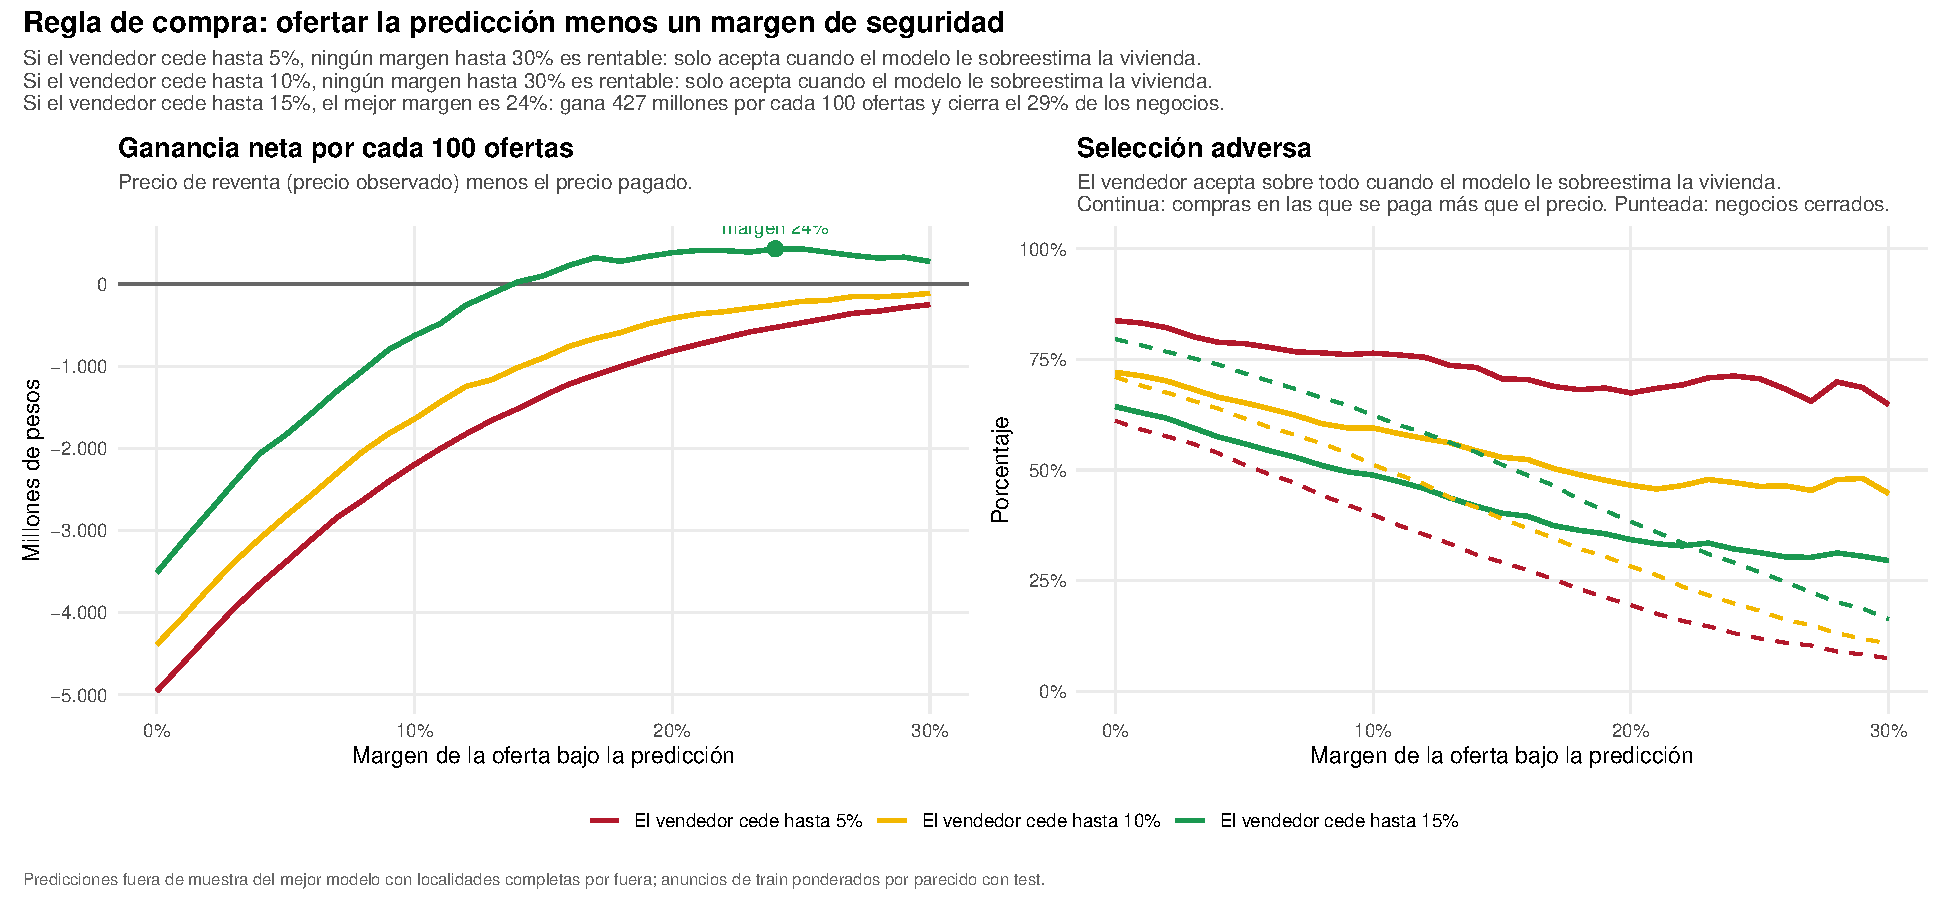
\includegraphics[height=0.8\textheight]{negocio_04_curva_margen.pdf}
  \lectura{En Chapinero, si el vendedor cede hasta \descuentomax, el margen más rentable es \mejormargen{}: \gananciacien{} millones por cada 100 ofertas, cerrando el \negociosmargen{} de los negocios.}
  \note{Selección adversa: los vendedores aceptan nuestra oferta sobre todo cuando el modelo les sobreestima la vivienda, porque en ese caso ofrecemos más de lo que vale. Con descuentos menores, \notadescuentos. Las curvas usan los \nchaptrain{} anuncios de Chapinero en train, por eso no son suaves. Los descuentos que acepta el vendedor son supuestos nuestros, no datos.}
\end{frame}

% C10. Semáforo de compra y recomendación
\begin{frame}{¿Compraríamos? Sí, como filtro y punto de partida, no como precio automático}
  \begin{columns}[c]
    \begin{column}{0.48\textwidth}\centering
      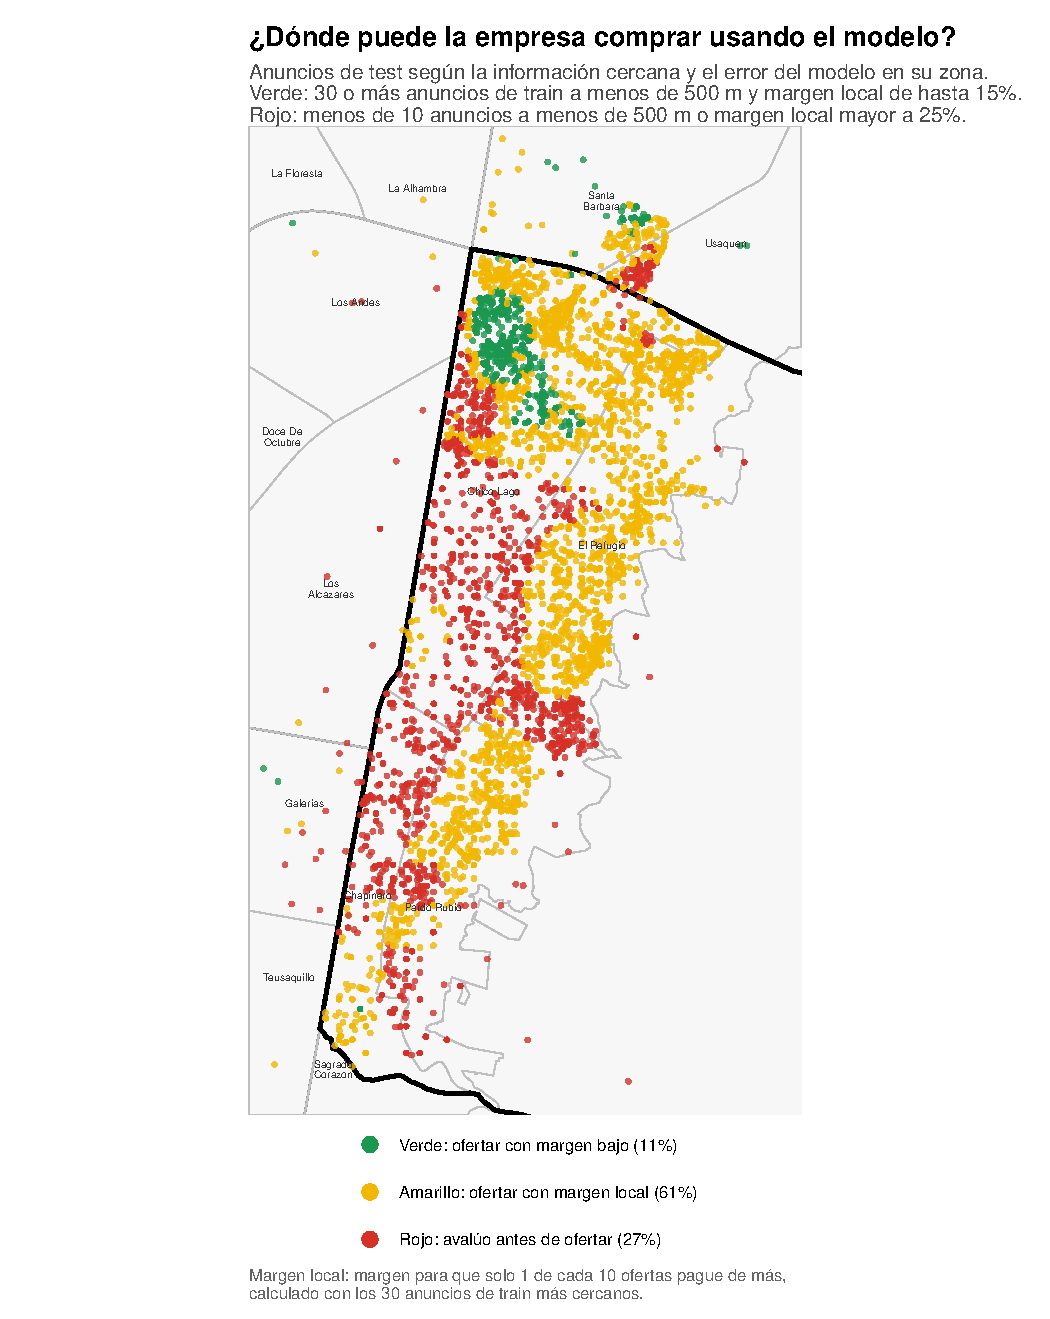
\includegraphics[height=0.84\textheight]{negocio_03_semaforo_test.pdf}
    \end{column}
    \begin{column}{0.5\textwidth}
      \textbf{\color{azul}Recomendación}
      \begin{enumerate}\small
        \item Usar la predicción como valor de referencia y ofertar alrededor de \margenchap{} por debajo.
        \item Verde (\pctverde): ofertar con margen bajo.
        \item Amarillo (\pctamarillo): ofertar con el margen de la zona.
        \item Rojo (\pctrojo): avalúo antes de ofertar.
        \item Monitorear las compras y reentrenar con los precios reales.
      \end{enumerate}
      \vspace{0.3em}
      {\small\color{gris}Riesgo principal: el vendedor acepta justo cuando el modelo le sobreestima la vivienda.}
    \end{column}
  \end{columns}
  \note{El semáforo combina dos cosas: cuántos anuncios de train hay cerca (si hay información) y qué tanto se equivoca el modelo en esa zona. El margen de \margenchap{} hace que solo 1 de cada 10 compras en Chapinero pague más que el precio. La compra automática no es rentable si el vendedor cede poco: los que aceptan son los que el modelo sobrevalora.}
\end{frame}


\end{document}
